\definecolor{gold}{rgb}{0.77,0.69,0.37}
\newlength{\hptitlewidth}
\newlength{\rationalh}
\newcommand{\hptitle}[2][\stockwidth]{%
  \setlength{\hptitlewidth}{#1}%
  \centering\color{white}%
  \vskip 3cm\resizebox{.95\hptitlewidth}{!}{\textls[100]{HARRY POTTER KAJ LA}}%
  \vskip 2mm%
  \color{gold}%
  \settoheight{\rationalh}{\resizebox{.95\hptitlewidth}{!}{\textls[20]{RACIECO}}}
  \resizebox{.95\hptitlewidth}{!}{\textls[20]{METODOJ DE}}%
  \vskip 2mm%
  \resizebox{.95\hptitlewidth}{!}{\textls[20]{LA RACIECO}}%
  \vskip 8mm%
  \color{white}%
  \resizebox{.5\hptitlewidth}{!}{\textls[50]{\scshape{}de Eliezer Yudkowsky}}%
  \vfill%
  \textls[50]{\scshape #2}%
  \color{black}%
  \vskip 1cm\ %
}
\providecommand{\fullvolumetitle}[1]{Libro #1: \volumetitle}

\ifcover%
\newpagecolor{black}\afterpage{\restorepagecolor}
\newcommand\BackgroundPic{
\put(0,0){%
\parbox[b][\paperheight]{\paperwidth}{%
\vfill%
\centering%
\includegraphics[width=\paperwidth,height=\paperheight,keepaspectratio]{cover0.jpg}%
\vfill%
}}}\AddToShipoutPicture*{\BackgroundPic}%
\AddToShipoutPicture*{\put(0,0){%
\parbox[b][\paperheight]{\paperwidth}{%
\hptitle{\fullvolumetitle{\volumenumber}}%
}}}%
\ %
\cleartorecto
\fi
\begin{center}
\thispagestyle{empty}
{\hpfont
\Huge\MakeUppercase{Harry Potter}\vspace*{0.5cm}

\Large\MakeUppercase{kaj la Metodoj de la Racieco} %

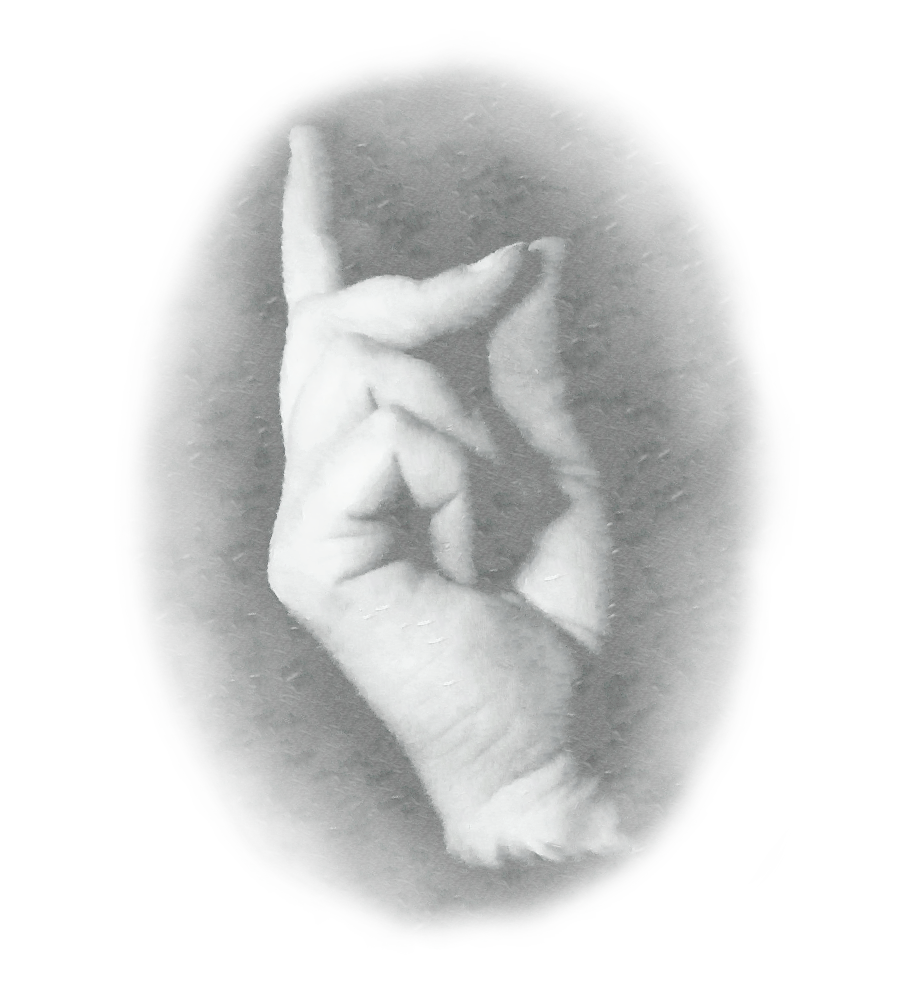
\includegraphics[scale=0.5]{bubble0.png}

\Large DE \vspace*{.25cm}

\huge \MakeUppercase{Eliezer Yudkowsky}%

\normalsize

\vspace*{1\baselineskip}
\fullvolumetitle{\volumenumber}
}
\vspace*{1\baselineskip}
\vspace*{1\baselineskip}
\vspace*{1\baselineskip}

Traduko el la angla lingvo al la esperanta per Emile Cadorel

\vspace{3cm}

\end{center}

\cleartoverso

\begin{center}
\vspace*{2cm}

\thispagestyle{empty}
Bazita sur la roluloj de 

\vspace*{.5cm}

\Large \MakeUppercase{J. K. Rowling} \normalsize

\vspace*{.5cm}

kaj ŝiaj libroj:

\vspace*{.5cm}

{
        \newcounter{books_list_counter}
        \def \hpBook #1{
                \addtocounter{books_list_counter}{1}
                \textit{Harry Potter kaj la #1} \par
                Jaro \numberstringnumesp{\value{books_list_counter}}a en Herpŭrko
                \smallskip\par
        }
        \hpBook{Filozofia Ŝtono}
        \hpBook{Ĉambro de Sekretoj}
        \hpBook{Malliberulo de Azkaban}
        \hpBook{Pokalo el Fajro}
        \hpBook{Ordeno de l'Fenikso}
        \hpBook{Reĝido de Duona Sango}
        \hpBook{Sanktaĵoj de l'Morto}
}
\end{center}
\cleartorecto% FIXME: For some reason, without this the contents ends up on a verso page (an extra blank page is added)
